\subsection{Tangent chord theorem}
\begin{namedframe}{Theorem}
	\small
	\begin{theorem}[Tangent chord theorem]
		Given that $TA$ is any chord of a circle and $PT$ is a tangent to the circle at $T$.
		If $C$ is a point on the circle chosen to be on the side of the chord opposite to the tangent then $\angle TCA = \angle PTA$.
	\end{theorem}
	\centering
	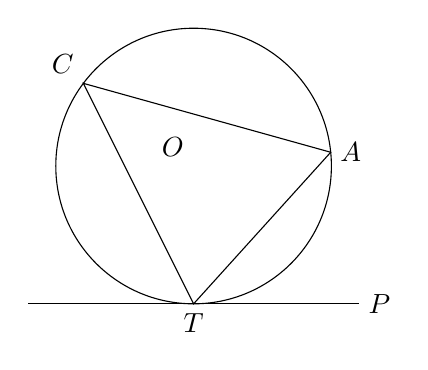
\begin{tikzpicture}[scale=0.35]
		\coordinate [label=above left:$O$](O) at (0,0);
		\coordinate [label=right:$P$](P) at (6,-5);
		\coordinate [label=below:$T$](T) at (0,-5);
		\coordinate (E) at (-6,-5);
		\coordinate [label=right:$A$](A) at (4.975, 0.499374608886);
		\coordinate [label=above left:$C$](C) at (-4, 3);

		\draw (O) circle (5);
		\draw (P) -- (T) -- (E);
		\draw (A) -- (C) -- (T) -- cycle;
	\end{tikzpicture}
\end{namedframe}
